\newpage
\chapter{Развертывание}
\subsection{Аппаратная конфигурация}
Для достижения минимальных затрат по закупке оборудования - система может
располагаться на одном физическом сервере. Однако данная схема не рекомендуется
из за ее ненадежности.

\begin{figure}[h]
\center{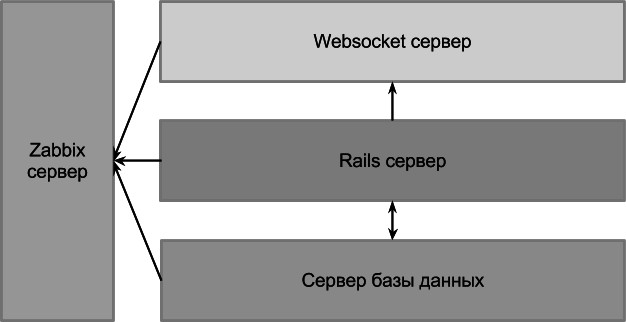
\includegraphics[width=1\linewidth]{hardware_configuration.eps}}
\caption{Схема связи между серверами}
\label{ris:hardware_configuration}
\end{figure}

На рисунке \ref{ris:hardware_configuration} изображена минимально рекомендуемая
схема серверов. При такой схеме кажный сервер выполняет свою задачу независимо
от других серверов:
\begin{enumerate}
  \item Websocket сервер обслуживает обмен сообщений между пользователями;
  \item Rails сервер обеспечивает работу непосредственно системы;
  \item Сервер базы данных обслуживает работу Postgresql базы;
  \item Zabbix сервер занимается мониторингом работы всех серверов.
\end{enumerate}

\subsection{Развертывание сайта}
Их схемы развертывания (рис. \ref{ris:deployment_sait}) видно что развертывание - это
многоэтапный процесс в котором важна последовательность этапов. Так же важно учитывать что приложение
считается обноленным только в случае если все этапы выполнены успешно. В случае
неуспешного выполения хотя бы одного из этапов необходимо обратить все
изменения. Исходя из анных фактов вытекает важно требования для системы
развертывания - транзакционность, т.е. любое изменение должно быть обратимо.

\begin{figure}[h!]
\center{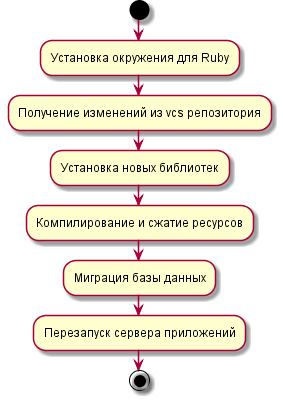
\includegraphics[width=0.5\linewidth]{deployment_sait.eps}}
\caption{Схема развертывания Ruby On Rails сайта}
\label{ris:deployment_sait}

% start
% 
% :Установка окружения для Ruby;
% :Получение изменений из vcs репозитория;
% :Установка новых библиотек;
% :Компилирование и сжатие ресурсов;
% :Миграция базы данных;
% :Перезапуск сервера приложений;
% 
% stop

\end{figure}

Для развертывания и обновления сайта на рабочем сервере существует библиотека
Capistrano. Данная библиотека позволяет настроить полностью контролируемый
процесс развертывания сайта.

Основные преимущества от использования данной библиотеки:
\begin{enumerate}
  \item поддержка транзакций и возможность обратить все изменения;
  \item гибкая настройка процесса за счет возможности выполнять любой удаленный
  \item код на сервере; 
  \item поддержка протокола ssh - необходимо для обеспечения безопасности; 
  \item интеграция с Ruby On Rails;
  \item развертывание на несколько серверов одновременно;
  \item установка окружения ruby.
\end{enumerate}

На данном этапе разработки библиотека не используется, так как нет необходимости
разворачивать приложение на рабочем сервере.

Рассмотрим инструкцию для запуска сайта в режиме разработчика.

В качестве операционой системы можно использовать любой UNIX-like дистрибутив.

Для начала нужно уставновить окружение для работы ruby, установку лучше всего
производить через rvm. Для работы проекта требуется ruby версии 1.9.3.

Далее необходимо установить базу данных Postgresql и создать пользователя в базе
данных с правами на создание баз данных. В конфигурационно файле
config/database.yml в секции development нужно выставить соответствующие логин и
пароль ждя подключения к базе данных.

Следующим шагом создадим непосредственно базу данных с помощью команды rake
db:create. База данных создана, но в ней нет необходимых таблиц. Чтобы добавить
таблицы в базу данных выполним rake db:migrate.

Для работы сайта создадим набор тестовых данных с помощью команды rake db:seed.

Запустим Websocket сервер с помощью команды rake wsserver.

Теперь можно запускать непосредственно сайт - rails s. После чего сайт будет
доступен по адресу \url{http://localhost:3000}.
\subsection{Nginx}
Архитектура работающего веб-сервера является двухуровневой. На первом уровне
находится HTTP-сервер, который перехватывает все HTTP запросы поступающие от
клиентов. В качестве такого сервера в нашем проекте используется бесплатный
сервер от Игоря Сысоева - nginx. Данный сервер длительное время он обслуживает
серверы многих высоконагруженных российских сайтов, таких как Яндекс, Mail.Ru,
ВКонтакте и Рамблер. Согласно статистике Netcraft nginx обслуживал или
проксировал 13.54\% самых нагруженных сайтов в мае 2013 года\footnote{
	\url{http://news.netcraft.com/archives/2013/05/03/may-2013-web-server-survey.html}
}.

Настройка сервера начинается с его установки. Это можно сделать обычными для
*nix систем способами - установить его через репозиторий пакетов, либо
скомпилировать из исходников с учетом особенностей конкретной рабочей машины.

Далее необходимо настроить конфигурацию для конкретного сайта (nginx позволяет
хостить множество сайтов). Для это в папке конфигурации надо создать файл с
именем сайта, как правило он расположен в папке
/etc/nginx/enabled-sites/site\_name.conf. В данном файле необходимо указать
полный URL сайта и номер порта. Также надо указать директорию в которой хранится
сайт. Как правило  для Ruby on Rails это /srv/site\_name/public.

С сервером второго уровня nginx связывается с помощью IPC-сокета, путь к 
которому указываются в конфигурационном файле сайта.
\subsection{Unicorn}
Сервер второго уровня получает поступающие запросы от сервера первого уровня,
выполняет их в среде Ruby on Rails, результат вычислений отдает в виде
стандартных веб-файлов (css, html, js) назад серверу первого уровня, который
отдает  их уже клиенту.

В качестве сервера второго уровня нами был выбран Unicorn. Данный сервер был
выбран за его популярность среди Ruby on Rails - разработчиков, что означает
наличие большого количества примеров файлов конфигурации, что ускоряет и
облегчает процесс развертывания.

Двухуровневая архитектура предоставляет возможность горизонтального
масштабирования системы. Например можно организовать кластер из серверов второго
уровня и распределять нагрузку между ними с помощью сервера первого уровня.

\subsection{Логи}
Аппаратная конфигурация системы предусматривает наличие нескольких физических
серверов. Для обеспечения дополнительного контроля за ними необходимо настроить
систему централизованного сбора логов. Данный подход позволит ускорить процесс
анализа логов за счет более удобного доступа или за счет использования утилит
для автоматического анализа логов.

\section{Бэкап}
Для обеспечения сохранности данных в системе важно создавать резервные копии
базы данных.

Существует множество решений для выполнения данной задачи. В системе
предполагается использовать решение для создания резервных копий на уровней
файловой системы - Bacula. Bacula достаточно проста в настройке и позволяет
создать распределенную систему для бэкапов.

В связке с Postgresql, Bacula позволяет создать PITR (point-in-time recovery)
бэкап - это механизм создания резервных копий, основанный на возможности
Postgresql создавать WAL-логи. WAL (Write Ahead Log) - это бинарные логи все
транзакций и запросов выполненных в базе данных. При верной настройке бэкап
будет отставать от основной базы всего на несколько минут.
\subsection{Администрирование}
При большом количестве независимых серверов возникает проблема контроля их
работы. Для обеспечения бесперебойной работы системы важно максимально быстро
выявлять проблемы в работе серверов и устранять эти проблемы.
	
Проблемы в работе серверов могут быть связаны с:
\begin{enumerate}
  \item низкой производительностью отдельных компонентов сервера (дисков, процессора);
  \item неправильной настройкой программного обеспечения или операционной
системы; 
  \item отказом оборудования;
  \item внешними факторами.
\end{enumerate}

Решение данной проблемы является настройка системы мониторинга, которая сможет
контролировать работу серверов и оповещать ответственного в случае неполадок.	

\subsubsection{Zabbix}
Zabbix\footnote{
	\url{http://www.zabbix.com/ru/}
} - это комплексное решение для мониторинга серверов различного типа,
включающее в себя:
\begin{enumerate}
  \item zabbix-agent - сервис устанавливаемый непосредственно на контролируемом сервере, позволяющий получать различные метрики работы сервера;
  \item zabbix-server - сервер собирает информацию с zabbix-agent’ов и сохраняет
ее в базу данных; сервер также занимается анализом поступающих данных и оповещает ответственных в случае если требуется вмешательство; 
  \item web интерфейс - позволяет производить настройку zabbix-server’а и
просматривать поступающие от серверов данные.
\end{enumerate}